\usepackage{nccmath}

\begin{document}

%----------------------------------------------------------------------------------------
%	TITLE PAGE
%----------------------------------------------------------------------------------------

\title[Personalization]{Talk 5: GADMM}
\date{2021-6-24}
\author[]{WEN Hao}

% \institute[北京航空航天大学] % Your institution as it will appear on the bottom of every slide, may be shorthand to save space
% {
% 数学科学学院 \\ % Your institution for the title page
% \medskip
% \textit{wenh06@gmail.com} % Your email address
% 北京航空航天大学 \\
% 数学科学学院 \qquad 北京航空航天大学
% }

% \logo{\includegraphics[height=1.5cm]{logo}}
% \logoii{\includegraphics[height=1cm]{logo2}}

% \date{\footnotesize 2021年4月13日} % Date, can be changed to a custom date

\setlength{\belowdisplayskip}{5pt} \setlength{\belowdisplayshortskip}{5pt}
\setlength{\abovedisplayskip}{5pt} \setlength{\abovedisplayshortskip}{5pt}

%------------------------------------------------

\begin{frame}
\titlepage % Print the title page as the first slide
\end{frame}

%------------------------------------------------
% Page 1

\begin{frame}
\frametitle{GADMM -- Origin}

Performance of distributed optimization algorithms is characterized by
\begin{itemize}
    \item computation time (complexity)
    \item communication time (especially in cross-device scenarios)
\end{itemize}

\pause
\vspace{0.6em}

Communication time is determined by
\begin{itemize}
    \item \# communication rounds
    \item {\color{green} \# channels (edges in the graph) per round}
    \item {\color{pink} bandwidth/power (data transmitted) per channel}
\end{itemize}

\pause
\vspace{0.6em}

And moreover, to fit the totally distributed (decentralized) clients network topology.

\end{frame}

%------------------------------------------------
% Page 2

\begin{frame}
\frametitle{GADMM -- Formulation}

The Group ADMM (GADMM) algorithm \cite{elgabli2020gadmm} considers the following clients network topology
\begin{figure}[H]
    \centering
    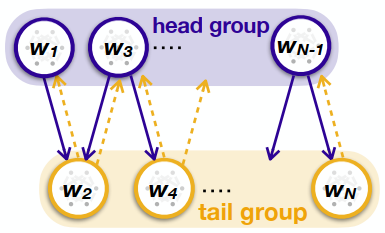
\includegraphics[width=0.45\textwidth,keepaspectratio]{images/GADMM.png}
\end{figure}
where all clients are divided into 2 groups, i.e. head group $\mathcal{N}_h$ and tail group $\mathcal{N}_t$. The problem hence is formulated as
\begin{align*}
    & \text{minimize} \quad \dfrac{1}{N} \sum\limits_{i=1}^N f_i(x_i) \\
    & \text{subject to} \quad x_i = x_{i+1}, \quad i=1,\cdots,N-1
\end{align*}

\end{frame}

%------------------------------------------------
% Page 3

\begin{frame}
\frametitle{GADMM -- Algorithm}

\begin{fleqn}
\begin{align*}
& \textbf{head group primal update (and transmit $\to$ tail group)}
\end{align*}
\begin{multline*}
    x_i^{k+1} = \argmin\limits_{x_i} \{ f_i(x_i) + \langle \lambda_{i-1}^k, x_{i-1}^k - x_i \rangle + \langle \lambda_{i}^k, x_{i} - x_{i+1}^k \rangle \\
    + \dfrac{\rho}{2}\lVert x_{i-1}^k - x_i \rVert^2 + \dfrac{\rho}{2}\lVert x_{i} - x_{i+1}^k \rVert^2 \}, \quad i \in \mathcal{N}_h
\end{multline*}
\begin{align*}
& \textbf{tail group primal update (and transmit $\to$ head group)}
\end{align*}
\begin{multline*}
    x_i^{k+1} = \argmin\limits_{x_i} \{ f_i(x_i) + \langle \lambda_{i-1}^k, x_{i-1}^{k+1} - x_i \rangle + \langle \lambda_{i}^k, x_{i} - x_{i+1}^{k+1} \rangle \\
    + \dfrac{\rho}{2}\lVert x_{i-1}^{k+1} - x_i \rVert^2 + \dfrac{\rho}{2}\lVert x_{i} - x_{i+1}^{k+1} \rVert^2 \}, \quad i \in \mathcal{N}_t
\end{multline*}
\begin{align*}
& \textbf{both groups dual update} \\
& \lambda_i^{k+1} = \lambda_i^k + \rho (x_i^{k+1} - x_{i+1}^{k+1})
\end{align*}
\end{fleqn}

\end{frame}

%------------------------------------------------
% Page 15

\begin{frame}
\frametitle{GADMM -- Remarks}

\begin{itemize}
    \item Consider the scenario with central (parameter) server, where the network is a star graph. It seems that the (vanilla) GADMM does {\color{red} NOT} communicate (per round) less than ADMM for a star graph. However, in the cross-device scenarios, where connection to central server might be slow.
    \item the (chain) topology is too restrictive. Any graph with a vertex of degree > 2 is not able to be fitted in the GADMM settings.
    \item more?
\end{itemize}

\end{frame}

%------------------------------------------------
% Page 15

\begin{frame}
\frametitle{Related Work -- M-ADMM}

In fact, $\exists$ previous work \cite{lu2017unified}\footnote{C. Lu, J. Feng, S. Yan, and Z. Lin, A unified alternating direction method of multipliers by majorization minimization, IEEE transactions on pattern analysis and machine intelligence, 2017} which proposed Mixed Gau\ss-Seidel and Jacobian ADMM (M-ADMM).

\vspace{0.6em}

M-ADMM partitions a {\color{red} multi-block problem} ($m$ blocks) into 2 groups $(1,\ldots,m')$ and $(m'+1,\ldots,m)$. The 2 groups update {\color{red} in serial}, while each block within one group updates {\color{red} in parallel}.

\end{frame}

%------------------------------------------------
% Page 15

\begin{frame}
\frametitle{Related Work -- M-ADMM}

Primal updates of M-ADMM are
\begin{fleqn}
\begin{multline*}
    x_i^{k+1} = \argmin_{x_i} \{ f_i(x_i) + \widetilde{\mathcal{L}}(x_1^{k},\ldots,x_i,\ldots,x_m^{k}, \lambda) \},\\
    1\leqslant i \leqslant m'
\end{multline*}
\begin{multline*}
    x_j^{k+1} = \argmin_{x_i} \{ f_i(x_i) + \widetilde{\mathcal{L}}(x_1^{k+1},\ldots,x_{m'}^{k+1},x_{m'+1}^{k},\\
    \ldots,x_j,\ldots,x_m^{k}, \lambda) \}, \quad m' < j \leqslant m
\end{multline*}
\end{fleqn}
where $\widetilde{\mathcal{L}}$ is some Lagrangian function, e.g. augmented Lagrangian, linearized Lagrangian, or {\color{red} majorant first-order surrogate} of $f_i$.

\end{frame}

%------------------------------------------------
% Page 15

\begin{frame}
\frametitle{CQ-GGADMM -- Enhanced GADMM}

\begin{figure}[H]
    \centering
    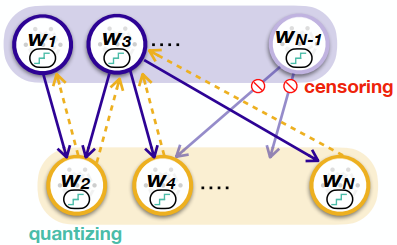
\includegraphics[width=0.5\textwidth,keepaspectratio]{images/CQ-GGADMM.png}
\end{figure}

\end{frame}

%------------------------------------------------
% Page 15

\begin{frame}
\frametitle{CQ-GGADMM -- Enhanced GADMM}



\end{frame}

%------------------------------------------------
% Page 15

\begin{frame}
\frametitle{Related Work -- LAG \& LASG}



\end{frame}

%------------------------------------------------
% Page 15

\begin{frame}[allowframebreaks]
\frametitle{References}

{\footnotesize
\bibliographystyle{ieeetr}
\bibliography{references}
}

\end{frame}

%------------------------------------------------

\end{document}
